\section{Umsetzung}
    \subsection{OCPP Standalone Server und Testframework}
        Alle gestellten Aufgaben benötigen OCPP Server um OCPP Kommunikation mit der Ladesäule auswerten zu können.

        Um den Server so flexibel wie möglich zu planen, wurde von meiner Seite entschieden, ihn nach "Clean Architecture" zu implementieren.
    \subsection{ERK Automatisierungstool}
        Das Automatisierungstool sollte laut der Aufgabenstellung in einer anderen bestehenden Tool integriert werden.
        Das bereits existierte Tool ist mit Electron geschrieben, daher um das Integrationsprozess so einfach wie möglich zu machen,
        wurde von meiner Seite entschieden auch mit Electron zu arbeiten. Das ERK Tool soll 2 vorgegebenen Schnittstellen benutzen:
        \begin{itemize}
            \item Die Kommunikationsschnittstelle zu der Autosimulator
            \item Die Kommunikationsschnittstelle zu dem Messgerät 
        \end{itemize}

        In dem bestehenden Tool wurde zur Begin der Umsetzung nur die Kommunikationsschnittstelle zur Autosimulator implementiert,
        die Kommunikationsschnittstelle zum Messgerät wurde von dem Messgeräthersteller vorgegeben. Die Schnittstelle wurde mit einem Pythonscript implementiert.
        Damit man die Schnittstelle nicht anpassen soll um verschiedene Fehler zu vermeiden, wird das Pythonscript vom Electronprogramm mit entsprechenden Parametern gestartet, 
        und danach wird nur die Konsoleausgabe empfängt und entsprechend ausgewertet. Am Ende des Ablaufs soll ein PDF Report entstehen, das alle wichitge Informationen
        über den Testablauf beinhaltet. Neben dem Report entstehen auch 2 weitere Ausgaben:
        \begin{itemize}
            \item Logs von dem Pythonscript
            \item Alle Messdaten
        \end{itemize}

        Die Logs können später benutzt werden um die Fehler im Pythonscript zu finden und um den Testablauf später nachmachen zu können.

        Die Messdaten werden aufbewahrt um später die Richtigkeit des Reports nachweisen und mit anderen Werkzeugen überprüfen zu können.

        Benutzten Werkzeuge:
        \begin{itemize}
            \item Typescript als Programmiersprach
            \item Svelte als Frontendframework
            \item Bulma als CSS Framework
        \end{itemize}

        \newpage
        Der komplette Testablauf:
        \begin{figure}[H]
            \centering
            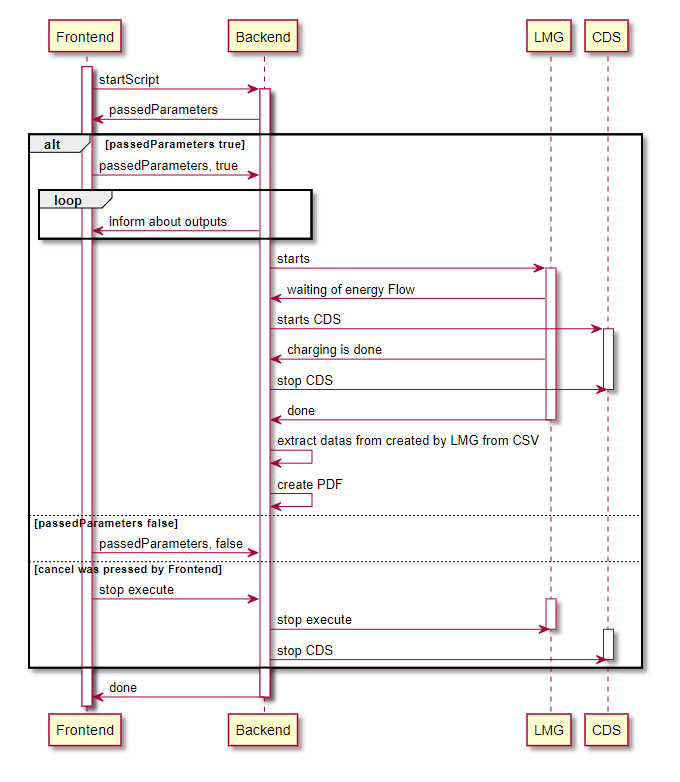
\includegraphics[width=1\textwidth]{./UML.png}
            \caption{Sequenzdiagramm ERK Tool}
            \label{fig:flow around cylinder}
            \source{Eigene Quelle}
        \end{figure}



        \newpage
        Beispiel des Reports: 
        \begin{figure}[H]
            \centering
            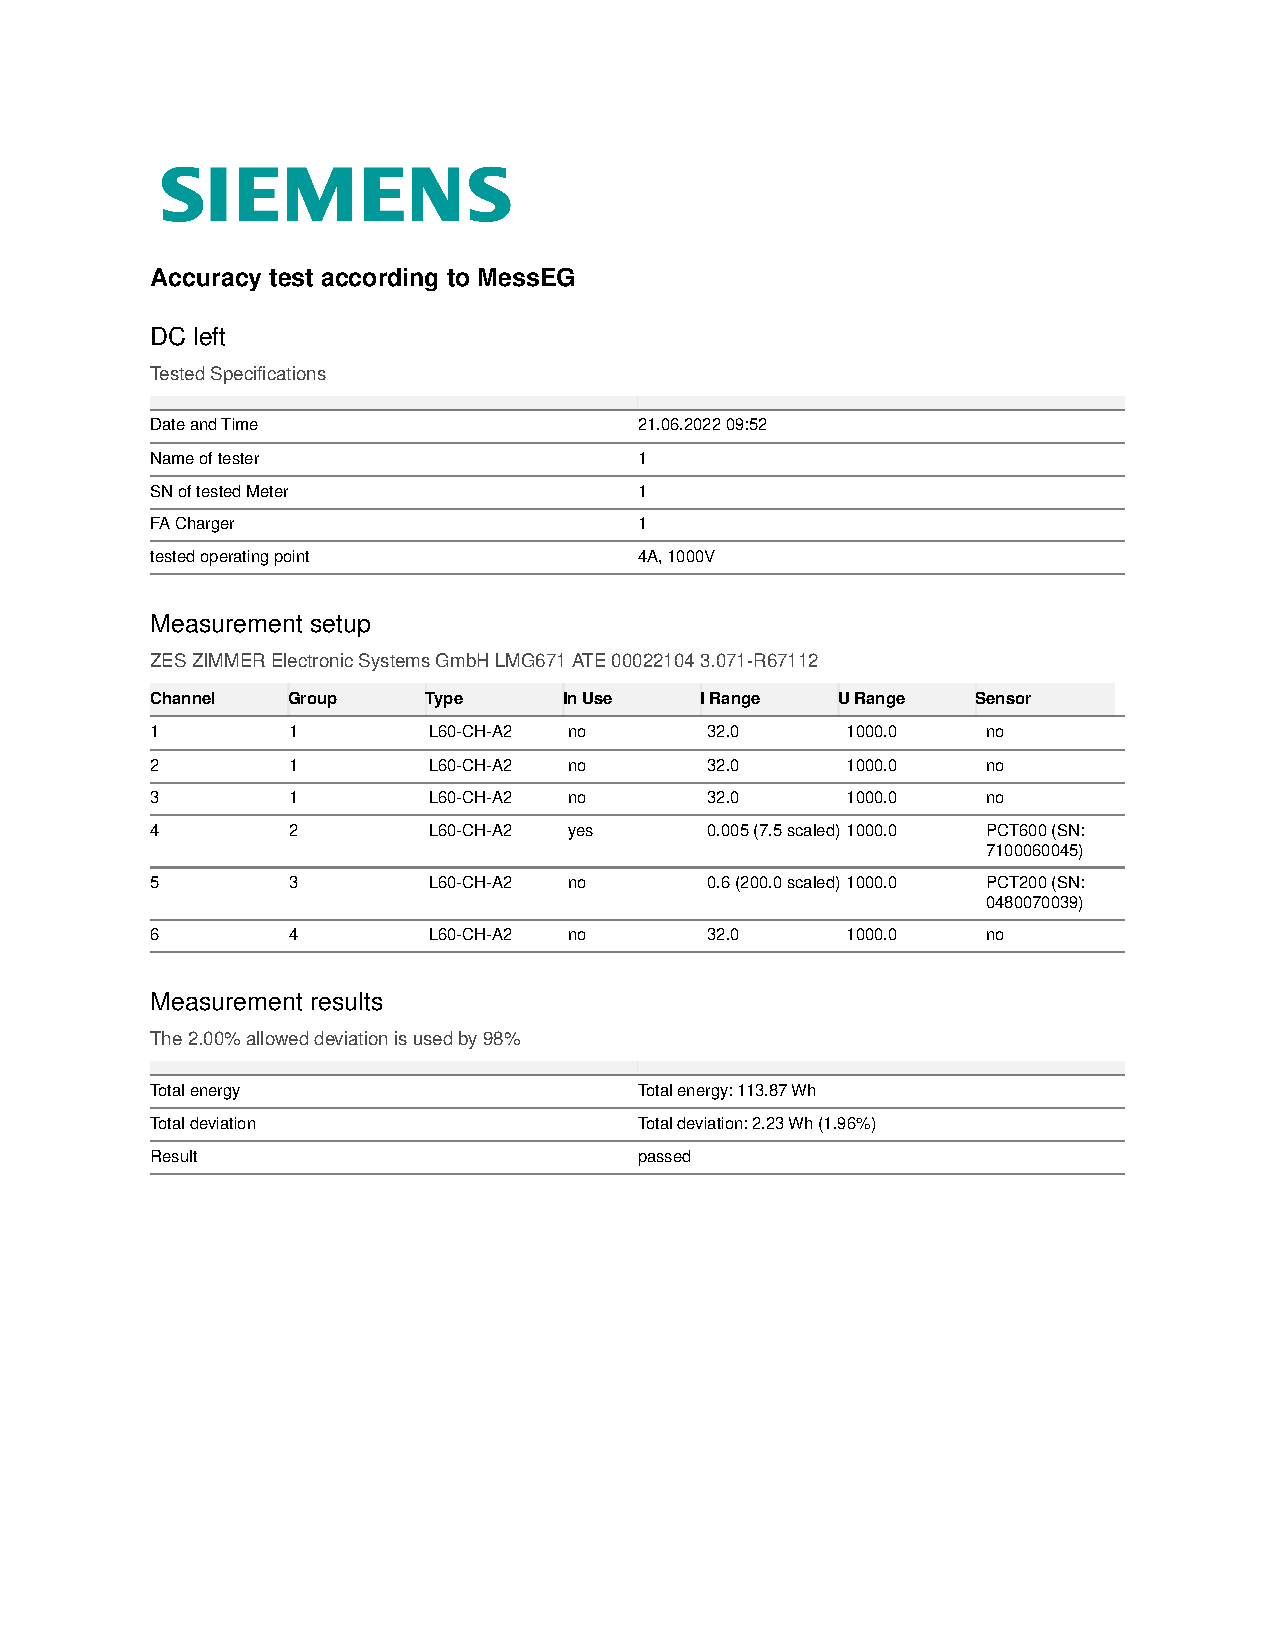
\includegraphics[width=1\textwidth]{./Report.pdf}
            \label{fig:flow around cylinder}
            \source{Eigene Quelle}
        \end{figure}